% don't remove the following lines, and edit the definition of \main if needed
\documentclass[../report.tex]{subfiles}
\providecommand{\main}{..}
\IfEq{\jobname}{\currfilebase}{\AtEndDocument{\biblio}}{}
% until here

\newcommand{\mlna}{\langle \ln\!A \rangle}
\newcommand{\nmu}{N_\mu}
\newcommand{\lnnmu}{\ln\!\nmu}
\newcommand{\xmax}{X_\text{max}}
\newcommand{\nmult}{N_\text{mult}}
\newcommand{\tocite}{{\bf REF}}
\newcommand{\si}[1]{\ensuremath{\text{#1}}}
\newcommand{\SI}[2]{\ensuremath{#1\,\si{#2}}}

\begin{document}

\section{Beyond...}

\subsection{Proton-oxygen collisions for cosmic ray research}

\begin{figure}
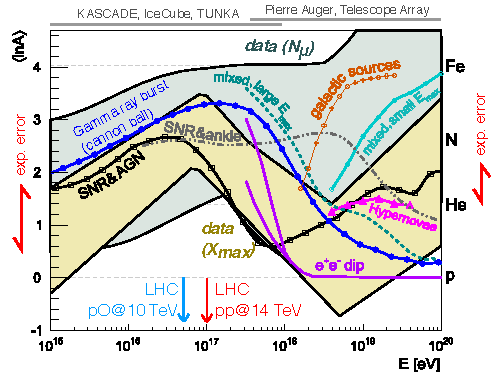
\includegraphics[width=0.5\textwidth,trim=5 -5 20 0]{\main/beyond/fig/lna_uncertainty.pdf}
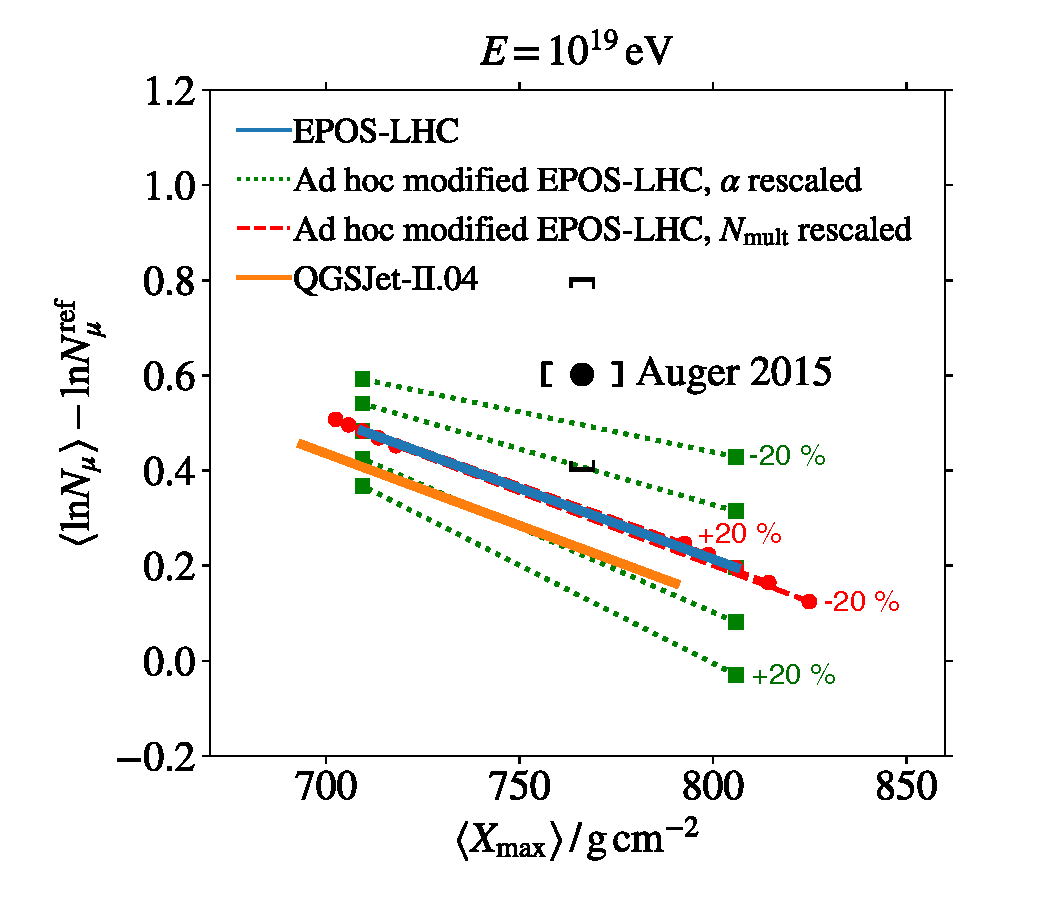
\includegraphics[width=0.5\textwidth,trim=-20 0 30 0]{\main/beyond/fig/epos_mod.pdf}
\caption{\emph{Left:} Elemental composition of cosmic rays, quantified by the mean-logarithmic-mass $\mlna$, as a function of cosmic ray energy $E$. The plot is based on the review of Kampert and Unger~\cite{kampert_cr_review}. Lines show predictions from astrophysical models of potential cosmic ray sources. Experimental measurements are shown as two bands. Each band is an envelope of data sets from different experiments. The bands are grouped by the air shower observable which was converted to $\mlna$, the number of muons $\nmu$ in the shower or the depth $\xmax$ of the shower maximum in the atmosphere. The width of each band is dominated by theoretical uncertainties in hadronic interaction models used in air shower simulations. The experimental uncertainty of 10-15\,\% is indicated at $10^{15}$ and $10^{20}$\,\si{eV} for comparison. \emph{Right:} Projected impact of measurements of hadron multiplicity $\nmult$ and the fraction $\alpha$ of neutral pions among all pions in p-O collisions at \SI{10}{TeV} on EPOS-LHC predictions for mean $\xmax$ and $\lnnmu$ in $10^{19}$\,\si{eV} air showers. The model lines represent all values that can be obtained for any mixture of cosmic nuclei from pure proton to iron. The point with brackets shows the Auger measurement with systematic uncertainties (statistical uncertainties are negligible). The dashed and dotted lines represent shifts in $\nmult$ and $\alpha$ of -20 to 20\,\% in steps of 10\,\% from the nominal value.}
\label{fig:cosmic_rays}
\end{figure}

The recent coincident observations of gamma rays and neutrinos from the flaring blazar TXS 0506+056 confirmed the conventional theory that active galactic nuclei produce high-energy cosmic rays\cite{IceCube:2018dnn}. This is a long awaited finding, but still leaves most in the dark about the dominant sources of ultra-high energy cosmic rays. Cosmic rays are charged and bent onto chaotic paths by magnetic fields in space. Their arrival directions are too isotropic to discriminate between source scenarios, but there are other ways.

Cosmic rays are nuclei from proton to iron (the fraction of heavier elements is negligible). The elemental composition of cosmic rays in a given energy interval is characteristic for different source scenarios. This is shown in Fig.~\ref{fig:cosmic_rays}, left-hand-side, where the mean-logarithmic-mass $\mlna$ of cosmic rays is plotted for several source scenarios. Above $10^{15}$\,\si{eV}, $\mlna$ can only be indirectly inferred, since cosmic rays are detected as air showers, particle cascades produced by nuclear collisions in the atmosphere. The two leading observables to infer $\mlna$ are the depth $\xmax$ of the shower maximum in the atmosphere, and the number $\nmu$ of muons produced.

Air shower simulations are required to predict these observables for different cosmic nuclei to infer the mass. The experimental uncertainties in the observables from leading experiments are at the level of 10-15\,\% in $\mlna$, which is sufficient to discriminate between source scenarios. However, a large uncertainty is added to the inference by the air shower simulations, and more precisely from the modeling of hadronic interactions in the shower. While predictions for the observable $\xmax$ have converged recently thanks to recent LHC measurements of the inelastic cross-section, the predictions for $\nmu$ still vary and are not consistent with $\xmax$. Most of the uncertainty originates from reports of the leading air shower experiments\cite{Aab:2014pza,Dembinski:2017zkb,Kokoulin:2009zz,AbuZayyad:1999xa,Aab:2014dua} that the muon number $\nmu$ is not consistently described by simulations. The measurement by the Pierre Auger Observatory is shown in Fig\.~\ref{fig:cosmic_rays}, right-hand-side. The simulations lack muons, which means that the data point is well above the predictions from all current hadronic interaction models. This produces conflicting estimates of the cosmic ray composition and destroys confidence in the interpretation of data.

Air shower simulations use specialized hadronic interaction models such as EPOS-LHC\cite{Werner:2005jf}, \mbox{QGSJet-II.04}\cite{Ostapchenko:2010vb}, and SIBYLL-2.3c\cite{Riehn:2017mfm}, which are designed to accurately describe nucleus-nucleus and soft-QCD interactions that produce particles in the forward direction, which dominate air-shower development. Since soft-QCD interactions cannot be described perturbatively, one uses phenomenological models based on Gribov-Regge theory and pomeron exchange, which need tuning and verification by reference measurements at colliders.

TODO: Talk about convergence in pp, but divergence in describing pO. Need to show another plot of hadron multiplicity and Eem/Ehad ratio with bands of current uncertainty.

\end{document}
